\documentclass[12pt]{article}
\usepackage[a4paper, left=3cm, right=3cm]{geometry}	% Per i margini
\usepackage[latin1]{inputenc}
\usepackage{amssymb}
\usepackage{color, xcolor}
\usepackage{listings}	% Per il codice.
\usepackage{graphicx}	% Per immagini e pdf.
\usepackage{amsthm}		% Per teoremi e dimostrazioni.
\usepackage{amsmath}
\usepackage[backend=bibtex, style=numeric, sorting=none, backref]{biblatex}
\usepackage{tabularx}


% --- Custom colors definitions --- %
\definecolor{mygreen}{rgb}{0,0.6,0}
\definecolor{mygray}{rgb}{0.5,0.5,0.5}


% --- LSTLISTING SETTING --- %
\lstset{ %
	backgroundcolor=\color{white},   			% choose the background color.
	basicstyle=\footnotesize\ttfamily,        % the size of the fonts that are used for the code
	breakatwhitespace=false,         			% sets if automatic breaks should only happen at whitespace
	breaklines=true,                 			% sets automatic line breaking
	captionpos=b,                    			% sets the caption-position to bottom
	commentstyle=\color{mygray},    			% comment style
	deletekeywords={...},            			% if you want to delete keywords from the given language
	escapeinside={\%*}{*)},          			% if you want to add LaTeX within your code
	extendedchars=true,              			% lets you use non-ASCII characters; for 8-bits encodings only, does not work with UTF-8
	frame=single,	                   			% adds a frame around the code
	keepspaces=true,                 			% keeps spaces in text, useful for keeping indentation of code (possibly needs columns=flexible)
	keywordstyle=\color{blue},       		% keyword style
	language=,                 				% the language of the code
	morekeywords={*,...},            			% if you want to add more keywords to the set
	numbers=left,                    			% where to put the line-numbers; possible values are (none, left, right)
	numbersep=5pt,                   			% how far the line-numbers are from the code
	numberstyle=\tiny\color{mygray}, 			% the style that is used for the line-numbers
	rulecolor=\color{black},         			% if not set, the frame-color may be changed on line-breaks within not-black text (e.g. comments (green here))
	showspaces=false,                			% show spaces everywhere adding particular underscores; it overrides 'showstringspaces'
	showstringspaces=false,          			% underline spaces within strings only
	showtabs=false,                  			% show tabs within strings adding particular underscores
	stepnumber=1,                    			% the step between two line-numbers. If it's 1, each line will be numbered
	stringstyle=\color{black},     			% string literal style
	tabsize=2,	                   			% sets default tabsize to 2 spaces
	title=\lstname                   			% show the filename of files included with \lstinputlisting; also try caption instead of title
}

\title{Relazione Sistemi Multi-Agente}
\author{Flavio Bizzarri, Riccardo Grieco, Marco Matarese}

\begin{document}

%\maketitle
% --- TITLE PAGE --- %

\thispagestyle{empty}

\begin{center}
	
\includegraphics[width=1\textwidth]{DIETI}
	
	\par\bigskip\par\bigskip\par\bigskip\par\bigskip\par\bigskip\par\bigskip\par\bigskip\par	% Per spazi
	
	{\huge Relazione Progetto di\\}
	{\huge Sistemi Multi-Agente\\}
	
	\par\bigskip\par\bigskip\par\bigskip\par\bigskip\par\bigskip\par\bigskip\par\bigskip\par	% Per spazi
	
	{\LARGE Flavio Bizzarri N97/0000281\\}
	{\LARGE Riccardo Grieco N97/0000286\\}
	{\LARGE Marco Matarese N97/0000280\\}
	
	\par\bigskip\par\bigskip\par\bigskip\par\bigskip\par\bigskip\par\bigskip	% Per spazi
	
	{\large A.A 2017/2018\par}
	
	%\includegraphics[width=0.5\textwidth]{}
\end{center}

%\newpage
\newpage

\tableofcontents

\newpage

\section{Introduzione}
%		** INTRODUZIONE **

Il presente progetto si prefige como scopo quello di realizzare un sistema multi-agente per il tracciamento di target in movimento in ambiente chiuso. Gli agenti previsti sono equiparabili a telecamere, le quali hanno un numero di funzioni limitate. Lo scopo principale degli agenti � quello di tenere i target tracciati il pi� possibile, per questo viene permesso loro di "passarsi" i target quando questi si allontanano dalla loro area di visione. L'applicazione � perzonalizzabile tramite file di configurazione, i quali permettono di specificare:
\begin{itemize}
	\item l'ambiente, tramite sua rappresentazione matriciale,
	\item le stanze, definite come rettangoli,
	\item gli agenti e la loro configurazione interna.
\end{itemize}
La figura seguente mostra l'interfaccia grafica dell'applicazione.

% Figura della mappa
\begin{figure}[h]
	\centering
	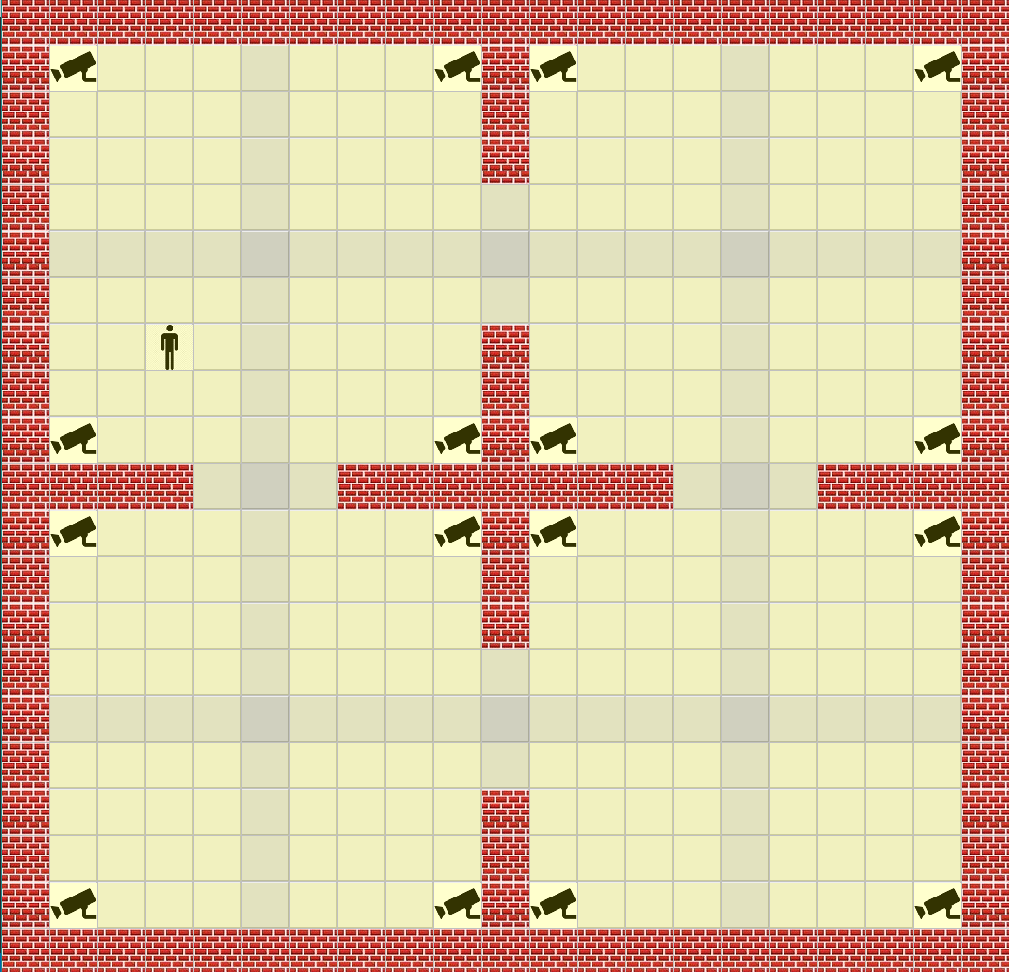
\includegraphics[width=0.5\linewidth]{mappa}
	\caption{Interfaccia grafica dell'applicazione in cui � visibile un target e i sedici agenti.}
	\label{fig:mappa}
\end{figure}

\newpage

\section{Architettura della Simulazione}
	\subsection{L'Ambiente}
	L'ambiente di simulazione, rappresentato dalla classe \textit{HouseEnv}, costituisce il fulcro dell'applicazione: i metodi di questa classe permettono di inizializzare le belief base degli agenti e di far percepire agli agenti gli spostamenti dei target.
Nel dettaglio permette di:
\begin{itemize}
\item caricare da file la posizione di ogni agente inizializzando la rispettiva classe java e belief base
\item stabilire per ogni agente l'area di visione e il numero di agenti che condividono una parte dell'area di visione
\item tenere traccia delle associazioni agente-target tracciato
\end{itemize}
L'aggiornamento delle belief base degli agenti � stato implementato attraverso un thread invocato ad ogni spostamento dei target che, dapprima procede ad eliminare ogni percept di ogni agente e, successivamente, definisce, a partire dalla configurazione del model, i nuovi percept da inserire nelle belief base.
	\subsection{La Vista}
	La vista dell'applicazione � rappresentata dalla classe \textit{HouseView} che estende GridWorldView. Quest'ultima, definita all'interno del package java associato a Jason, prevede che l'ambiente, dunque lo spazio di simulazione, sia discretizzato attraverso una griglia di posizioni. In particolare permette di disegnare in una griglia di posizioni attraverso l'override del metodo \texttt{public void draw(Graphics g, int x, int y, int object)}.

L'implementazione standard di Jason prevede ad ogni cambiamento di posizione di ridisegnare l'intera area Canvas: per evitare fastidiosi flickering dovuti a spostamenti continui dei target si � scelto di avere memoria delle vecchie posizioni occupate e ridisegnare unicamente l'area precedente e la nuova.

	\subsection{Il Modello}
	Il modello, rappresentato dalla classe \textit{HouseModel} rappresenta il collante tra l'environment e la vista. Infatti contiene i riferimenti di ogni target, agente e degli ostacoli presenti all'interno dell'ambiente simulato. 
I compiti preliminari dell'ambiente sono:
\begin{itemize}
	\item caricare da file la descrizione dell'ambiente e in particolare numero e composizione delle stanze
	\item istanziare ad intervalli regolari un nuovo target fino al raggiungimento del limite massimo specificato
	\item costruire il grafo delle posizioni calpestabili dai target e fornirne un iteratore
\end{itemize}
Inoltre il model provvede a riempire e aggiornare una matrice di interi che rappresenta la griglia delle posizioni degli oggetti all'interno dell'ambiente utilizzata dalla view per l'aggiornamento del Canvas e informa l'environment della presenza di nuovi target.
	
	\newpage

\section{Agenti e Target}
	\subsection{Il Meccanismo d'Asta}
	%		** MECCANISMO D'ASTA **

Le aste rappresentano l'elemento fondamentale dell'interazione fra gli agenti. Tramite le aste, gli agenti possono cedere e acquisire nuovi target da tracciare. Ci sono due momenti in cui un agente pu� bandire un'asta:
\begin{itemize}
	\item quando un target attualmente tracciato � in procinto di abbandonare la sua area di visione; in tal caso diremo che lo sta perdendo
	\item quando, dopo aver ricevuto notifica sulla vincita di un'asta precedente, cerca di cedere il target che gi� sta tracciando.
\end{itemize}
Il protocollo d'asta implementato prevede l'utilizzo di aste \textit{First-Price Sealed-Bid}: un tipo d'asta \textit{one-shot} a busta chiusa. 

Il valore della puntata di un'asta viene specificato attraverso la seguente funzione, la quale � implementata attraverso l'azione interna \textit{calculateBid}.

Siano $A$ l'agente che deve effettuare la puntata per il nuovo target $t_n$, $t$ l'eventuale target che $A$ sta gi� tracciando, $N_A$ il numero di vicini di $A$, $dist$ una funzione distanza (ad es. distanza Euclidea) fra un agente ed il target che sta tracciando e $k \in \mathbb{N}$ tale che $k \gg \max dist(A, t)$, allora:
\begin{center}
	$$
	b(A) =
	\begin{cases} 	
	\frac{(2 dist(A,t) - dist(A, t_n)) - k}{N_A} & \mbox{se }A \mbox{ sta tracciando }t \\ \\
	\frac{dist(A,t)^{-1} + k}{N_A} & \mbox{ altrimenti.}
	\end{cases} 
	$$
\end{center}
La funzione cos� definita soddisfa i seguenti vincoli:
\begin{itemize}
	\item gli agenti "liberi" vincono sempre sugli agenti "occupati"
	\item fra agenti "liberi" vince sempre il pi� vicino al target
	\item fra agenti "occupati" vince sempre l'agente che ha pi� vicino il target e contemporaneamente ha il target attualmente tracciato pi� lontano
	\item a parit� di tutto, vince chi ha meno vicini.
\end{itemize}

Una tipica interazione fra agenti in un contesto d'asta � rappresentata dal seguente \textit{sequence diagram}.

% Figura sequence diagram
\begin{figure}[htp]
	\centering
	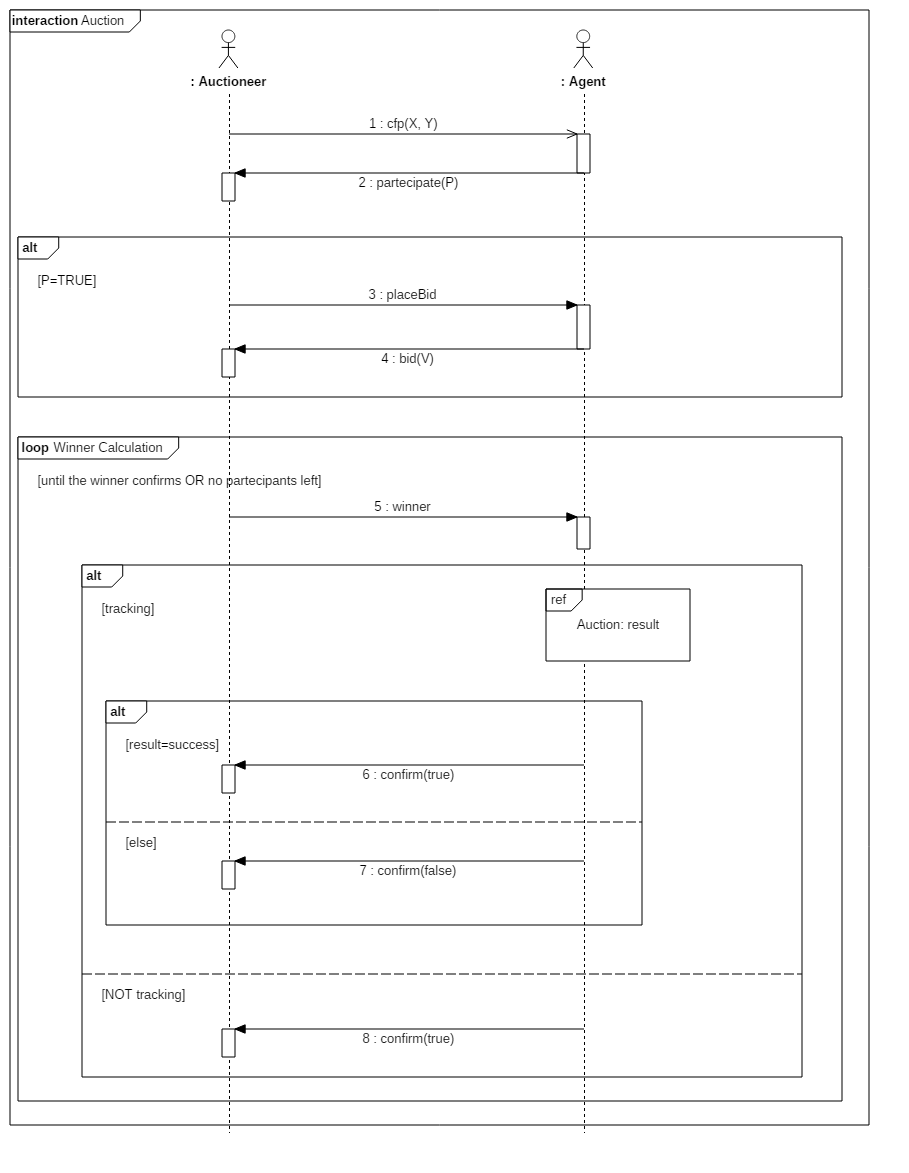
\includegraphics[width=\linewidth]{Auction}
	\caption{Protocollo d'asta.}
	\label{fig:auction}
\end{figure}

	\subsection{Comportamento degli Agenti}
	%		** COMPORTAMENTO DEGLI AGENTI **


Ogni agente viene inizializzato per mezzo di una serie di \textit{percept}, i quali vengono estratti da un file JSON di configurazione. Gli agenti telecamera hanno posizione fissa e una porzione di spazio a loro visibile. Tale area di visione pu� essere sovrapposta con quella di altri agenti, ma nessuno di questi ha informazioni sui parametri degli altri. Fra i percept iniziali troviamo anche quello riferito al numero di vicini, cio� il numero di agenti con cui un particolare agente pu� comunicare. Per comodit� di utilizzo del framework di simulazione, questi percept iniziali vengono trasformati in \textit{mental notes} dell'agente.

Ogni agente, inoltre, tiene memoria di un intero progressivo con il quale etichetta i target che scopre. I target, infatti, vengono identificati dagli agenti attraverso due attributi: nome dell'agente che lo ha scoperto, un numero progressivo che indica il numero di target che quel particolare agente ha scoperto fino a quel momento. Si dice che un agente scopre un target quando lo percepisce nella sua area di visione e, dopo aver chiesto ai suoi vicini se stanno tracciando un target in quella posizione, ottiene solo risposte negative.

\'E stata prevista una sola regola per gli agenti: amInterested(X,Y), la quale � vera se l'agente � interessato ad un target in posizione (X,Y).\\ \\

La seguente tabella riassume le \textit{belief} degli agenti.
\begin{center}
\begin{tabularx}{\textwidth}{| l | X |}
	\hline
	\textbf{Belief}						&	\textbf{Descrizione} \\ \hline
	numberOfAgents(N)					&	Il numero di agenti totali � N. \\ \hline
	noNeighbors(N)						&	L'agente condivide aree di visione con N altri agenti. \\ \hline
	myPosition(X,Y)						&	La posizione dell'agente nell'ambiente � (X,Y).\\ \hline
	canSee(A,B,C,D)						&	L'ambiente pu� vedere il rettangolo specificato dai punti (A,B) e (C,D). \\ \hline
	progressiNo(N)						&	Numero progressivo dell'agente per l'etichettatura di un nuovo target. \\ \hline
	losingTarget(Ag,Tid,X,Y)			&	L'agente sta perdendo il target identificato con (Ag,Tid) nella posizione (X,Y). \\ \hline
	auctionOnGoing(Ag,Tid,X,Y)			&	L'asta per il target (Ag,Tid) che ha bandito l'agente � ancora in corso. \\ \hline
	numberOfPartecipants(Ag,Tid,N)		&	Il numero di partecipante all'asta per il target (Ag,Tid) � N. \\ \hline
	partecipate(Ag,Tid,V)[source(S)]	&	V indica se l'agente S partecipa all'asta per il target (Ag,Tid). \\ \hline
	bid(Ag,Tid,V)[source(S)]			&	V indica la puntata effettuata dall'agente S nell'asta per il target (Ag,Tid). \\ \hline
	winner(Ag,Tid,X,Y)					&	Indica che l'agente � il vincitore dell'asta per il target (Ag,Tid). \\ \hline
	target(X,Y)							&	L'agente ha scoperto un nuovo target in posizione (X,Y). \\ \hline
	tracking(Ag,Tid,X,Y)				&	L'agente sta tracciando il target (Ag,Tid) in posizione (X,Y). \\ \hline
	alreadyTracking(X,Y,T,I)[source(S)]	&	T indica se l'agente S sta gi� tracciando il target in posizione (X,Y). I indica se l'agente S � interessato al target in posizione (X,Y). \\ \hline
\end{tabularx}
\end{center}

\newpage


La seguente tabella riassume i \textit{goal} degli agenti.

\begin{center}
	\begin{tabularx}{\textwidth}{|l |X |}
		\hline
		\textbf{Goal}					&	\textbf{Descrizione}	\\ \hline
		findWinner(Ag,Tid)				&	Calcola il vincitore di un'asta tra i partecipanti rimanenti. \\ \hline
		confirm(Ag,Tid,C)[source(S)]	&	In base alla conferma/rifiuto di vittoria dell'agente S, indicata da C, agisce come da protocollo d'asta. \\ \hline
		clearAuction(Ag,Tid)			&	Elimina i beliefs relativi all'asta per il target (Ag,Tid) dalla belief base dell'agente. \\ \hline
		cfp(Ag,Tid,X,Y)[source(S)]		&	Dichiara l'intenzione dell'agente di partecipare all'asta per il target (Ag,Tid) in posizione (X,Y). \\ \hline
		placeBid(Ag,Tid,X,Y)[source(S)]	&	Calcola la puntata per l'asta per il target specificato e la invia al banditore S. \\ \hline
		tellMeTracking(X,Y)[source(S)]	&	Comunica a S se l'agente sta attualmente tracciando il target in posizione (X,Y). \\ \hline
	\end{tabularx}
\end{center}

% perch� non askAll o askOne? non posso gestire il caso in cui tutti rispondono negativamente 
	\subsection{Comportamento dei Target}
	%		** COMPORTAMENTO DEI TARGETS **

I targets hanno un comportamento molto semplice: appaiono in maniera casuale nella mappa e si muovono fra le diverse stanze. Lo \textit{spawn} dei target � gestito dall'omonima classe Target, la quale attende un periodo di tempo prefissato prima di far apparire un nuovo target. Nella classe Target viene inoltre specificato il numero massimo di target permessi. Lo spawn � gestito in modo da far apparire i target solo in punti liberi della mappa. Il movimento dei target prevede due fasi distinte:
\begin{itemize}
	\item calcolo della destinazione,
	\item raggiungimento della destinazione.
\end{itemize}
Al primo passo, viene scelto una locazione a caso fra quelle appartenenti alle stanze diverse rispetto a quella in cui si trova attualmente il target, e viene impostata come destinazione. I target raggiungono la loro destinazione un passo alla volta: ogni passo differisce dall'altro di un periodo di tempo prefissato.
	
	\newpage
	
\section{Risultati}
%		 ** RISULTATI **

Le figure~\ref{fig:room} e~\ref{fig:console} mostrano un caso potenzialmente problematico di situazione ciclica. In tale situazione, tutti e quattro gli agenti della stanza sono occupati a tracciare un target diverso e l'inizio di un'asta potrebbe scatenare una reazione a catena senza fine. Utilizzando il protocollo d'asta implementato, la situazione si risolve con uno scambio di target.

% Figura della mappa
\begin{figure}[htp]
	\centering
	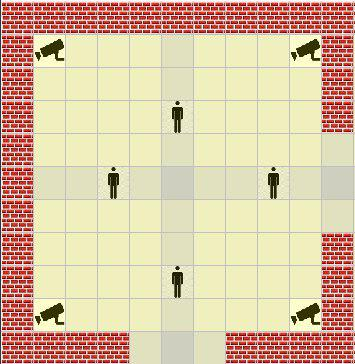
\includegraphics[width=0.3\linewidth]{room}
	\caption{Configurazione dei target ciclica.}
	\label{fig:room}
\end{figure}

% Figura della mappa
\begin{figure}[htp]
	\centering
	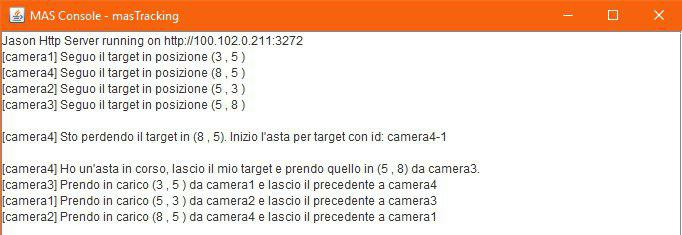
\includegraphics[width=0.7\linewidth]{console}
	\caption{Output ricevuto con la configurazione mostrata in Figura 3.}
	\label{fig:console}
\end{figure}

Le figure~\ref{fig:room2} e~\ref{fig:console2} mostrano un altro caso particolare. Nello scenario mostrato l'agente 2 vince l'asta per il target che l'agente 1 sta perdendo. Tuttavia, egli non riesce a cedere il suo attuale target e, di conseguenza, rifiuta la vincita. L'agente 1 allora ricalcola come vincitore l'agente 4, il quale riesce a cedere il suo attuale target ad un agente della stanza a fianco.

% Figura della mappa
\begin{figure}[htp]
	\centering
	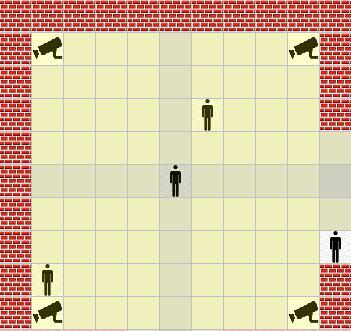
\includegraphics[width=0.3\linewidth]{room2}
	\caption{Configurazione dei target particolare.}
	\label{fig:room2}
\end{figure}

% Figura della mappa
\begin{figure}[htp]
	\centering
	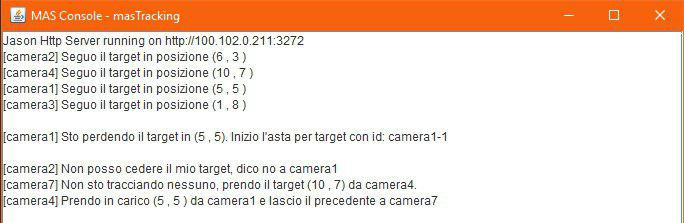
\includegraphics[width=0.7\linewidth]{console2}
	\caption{Output ricevuto con la configurazione mostrata in Figura 3.}
	\label{fig:console2}
\end{figure}

Le figure~\ref{fig:room3} e~\ref{fig:console3} mostrano il fallimento di un'asta. Infatti, tutti e tre i partecipanti candidati non possono cedere il proprio target. Il banditore mantiene quindi il proprio target nella speranza che rimanga ancora nel suo campo visivo.

% Figura della mappa
\begin{figure}[htp]
	\centering
	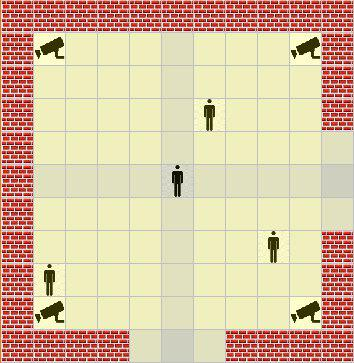
\includegraphics[width=0.3\linewidth]{room3}
	\caption{Configurazione dei target particolare.}
	\label{fig:room3}
\end{figure}

% Figura della mappa
\begin{figure}[htp]
	\centering
	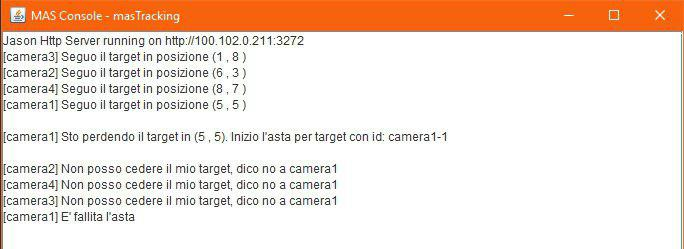
\includegraphics[width=0.7\linewidth]{console3}
	\caption{Output ricevuto con la configurazione mostrata in Figura 3.}
	\label{fig:console3}
\end{figure}

\newpage

La tabella seguente riassume, al variare del numero di target, le seguenti statistiche:
\begin{itemize}
	\item numero medio di aste effettuate,
	\item numero medio di aste non andate a buon fine,
	\item numero medio di step in cui un target non � tracciato.
\end{itemize}
\begin{center}
\begin{tabular}{| c | c | c | c |}
	\hline
	\textbf{No Target}	&	\textbf{No Aste}	&	\textbf{No Aste Fallite}	&	\textbf{No Target Persi} \\ \hline
	1	&	20	&	0	&	3	\\ \hline
	2	&	85	&	7	&	19	\\ \hline
	3	&	152	&	17	&	54	\\ \hline
	4	&	190	&	18	&	120	\\ \hline
	5	&	366	&	45	&	145	\\ \hline
\end{tabular}
\end{center}

I dati raccolti evidenziano come simulare con spazi stretti e aree di visione in comune piccole, porta gli agenti a perdere abbastanza spesso i loro target; soprattutto perch� questi hanno sviluppato una particolare abilit� a camminare sui bordi delle aree di visione.

In generale, per poter ottenere una stima migliore della bont� del sistema, bisognerebbe utilizzare un ambiente di simulazione con una risoluzione dello spazio maggiore. Inoltre, da un'analisi real time del comportamento del sistema stesso, � emersa la necessit� di una logica decisionale pi� intelligente per il riconoscimento dell'allontanamento dei target e della sua possibile perdita.

\end{document}
